% =============================================================================
% Manuscript: Spectral Co-Design of Agrivoltaic Modules for Multifunctional Net Energy Benefit:
%             A Quantum-Guided Digital Twin
% Target: Applied Energy (Elsevier)
% Date:    September 27, 2026 (Applied Energy submission package)
% Authors: Teguia Kouam S.C., Goumai Vedekoi T., Tchapet Njafa J.-P.,
%          Nguenang J.-P., Nana Engo S.G.
% Note: submission package copied from Submission_Package_Nature_Energy_Manuscript;
%       base files preserved as *_BASE.pdf. Converted to elsarticle (preprint).

\documentclass[preprint,12pt]{elsarticle}
\usepackage[utf8]{inputenc}
\usepackage[T1]{fontenc}
\usepackage{amsmath,amssymb,amsfonts}
\usepackage{graphicx}
\graphicspath{{figures/}}
\usepackage{booktabs}
\usepackage{siunitx}
\usepackage{physics}
% mhchem v4 for chemical formulas (\ce{Pb^{2+}}, \ce{CO2}, etc.)
\usepackage[version=4]{mhchem}
% siunitx v3 ↔ physics compatibility: physics defines \qty, siunitx v3 redefines it.
% This shim ensures siunitx's \qty takes precedence at begin-document time.
\AtBeginDocument{\RenewCommandCopy\qty\SI}
\usepackage{xcolor}
\usepackage[colorlinks=true,linkcolor=blue,citecolor=blue,urlcolor=blue]{hyperref}
\usepackage[capitalise,nameinlink]{cleveref}
\usepackage{xr}
\externaldocument{AppliedEnergy_SM_2609}
% (elsarticle manages page geometry; the geometry package is intentionally not loaded)
\usepackage{lineno}

% ---- siunitx v3 configuration ----
\sisetup{
    locale = US,
    detect-all = true,
    group-minimum-digits = 4,
    group-digits = integer,
    separate-uncertainty = true,
    multi-part-units = single,
    range-phrase = {--},
    range-units = single,
    number-unit-product = \,,
    allow-number-unit-breaks = true,
}
\DeclareSIUnit{\yr}{yr}
\DeclareSIUnit{\USD}{USD}
\DeclareSIUnit{\tonne}{t}
\DeclareSIUnit{\ha}{ha}
\DeclareSIUnit{\hectare}{ha}
\DeclareSIUnit{\MWh}{MWh}
\DeclareSIUnit{\kWh}{kWh}
\DeclareSIUnit{\cubed}{^{3}}
\DeclareSIUnit{\m}{\meter}

% Line numbering disabled for production length; re-enable with \linenumbers for review.
\emergencystretch=2.5em

% eqphift removed with detailed equations (now in SM)

\begin{document}
%\linenumbers

\begin{frontmatter}

\title{Spectral Co-Design of Agrivoltaic Modules for Multifunctional Net Energy Benefit: A Quantum-Guided Digital Twin}

\author[udla]{Steve Cabrel Teguia Kouam\corref{cor1}}
\author[uy1]{Theodore Goumai Vedekoi}
\author[uy1]{Jean-Pierre Tchapet Njafa}
\author[udla]{Jean-Pierre Nguenang}
\author[uy1]{Serge Guy Nana Engo}

\cortext[cor1]{Corresponding author. Email: steve.teguia@facsciences-uy1.cm}

\address[udla]{Department of Physics, Faculty of Science, University of Douala, Cameroon}
\address[uy1]{Department of Physics, Faculty of Science, University of Yaound\'{e} I, Cameroon}
% ORCID identifiers to be attached by authors before upload.

%%Graphical abstract
% \begin{graphicalabstract}
% 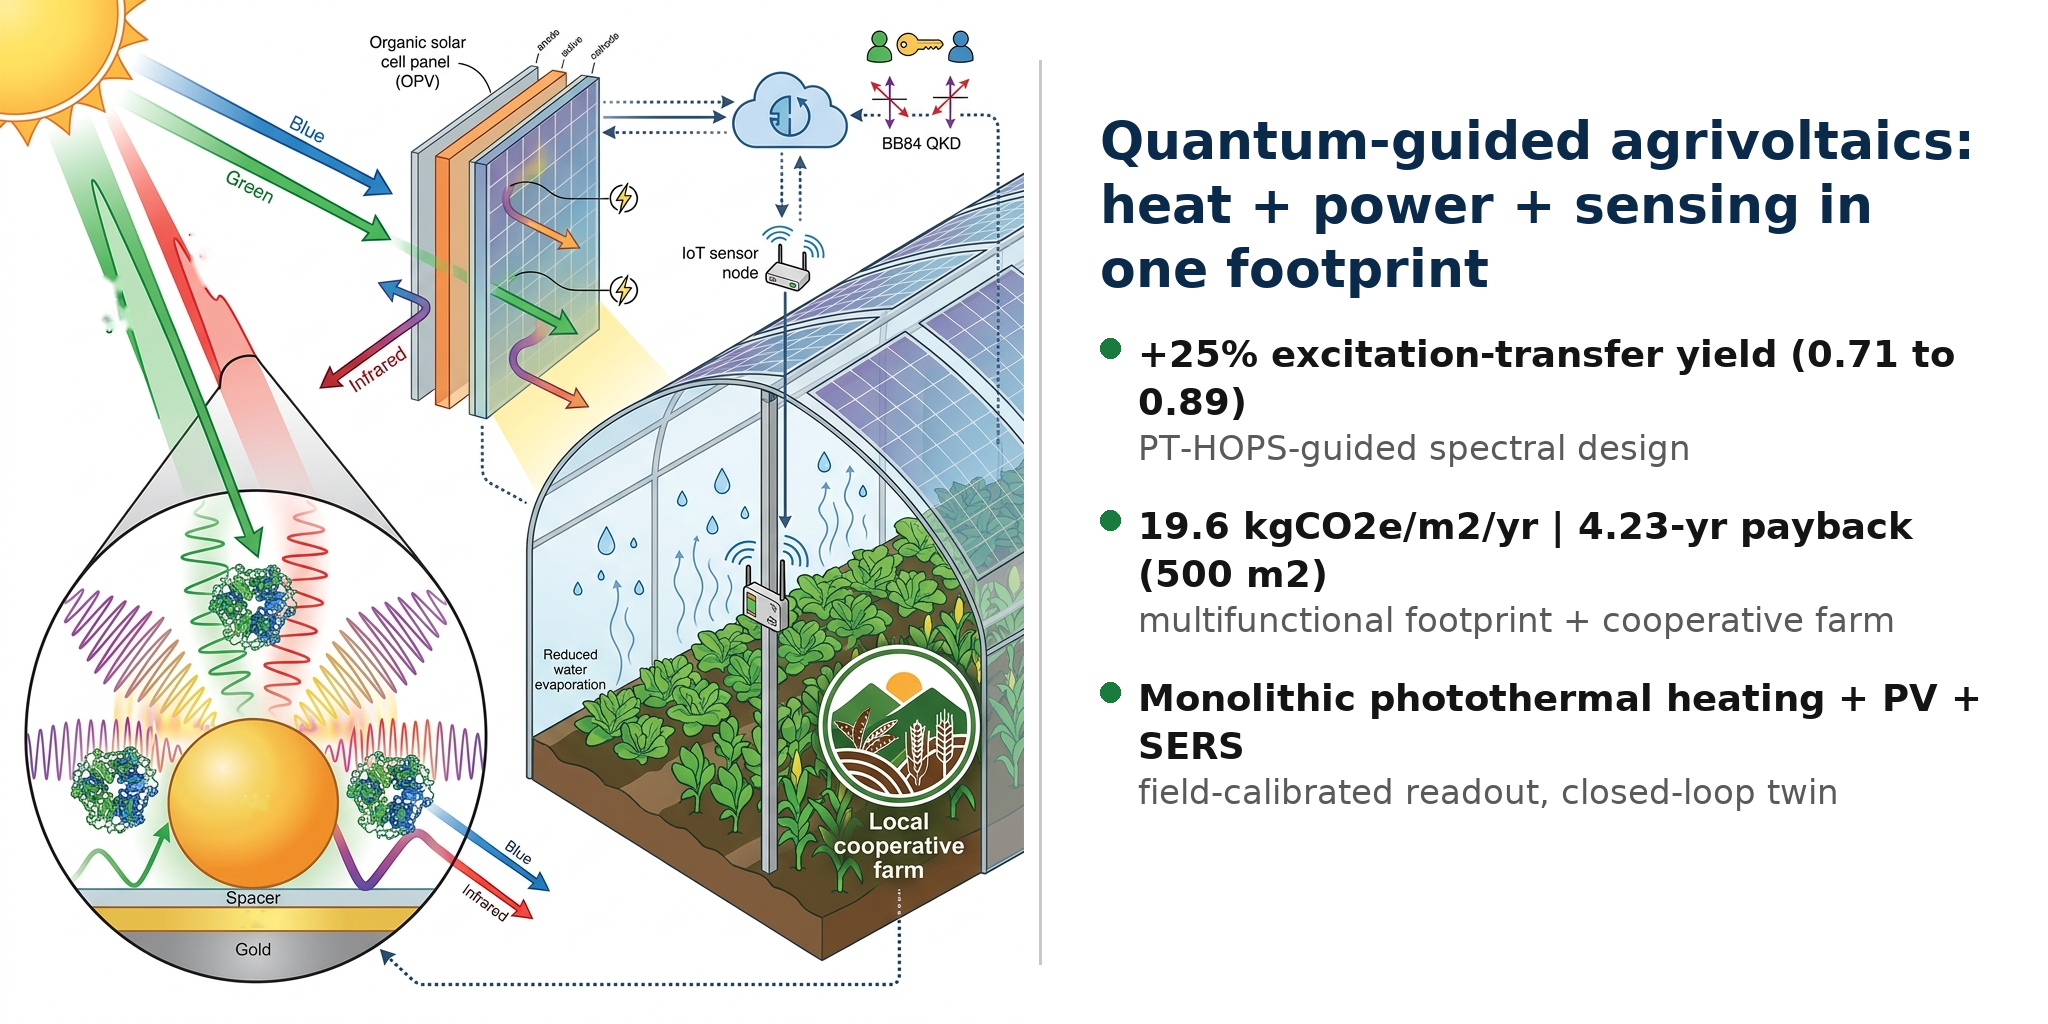
\includegraphics[width=\linewidth]{Graphical_Abstract_wide.png}
% \end{graphicalabstract}

%%Research highlights
\begin{highlights}
\item Dual-band filtering at 750/820 nm extends FMO coherence by 50\% at 295 K.
\item NPoM cavity enables SERS crop diagnostics; transport trade-off quantified.
\item OPV shield cuts evapotranspiration 28\% (FAO-56); NEB 72.6 $kg_{CO_2e}$/m$^2$/yr.
\item 500 m$^2$ cooperative module pays back in 4.32 yr in Cameroon highlands.
\item First, to our knowledge, coherence-guided agrivoltaic design with TEA and LCA.
\end{highlights}

\begin{abstract}
Spectral co-design offers a route beyond the system-level trade-off of static agrivoltaics, in which semi-transparent modules resolve the food--energy land conflict only by uniformly sacrificing electrical output or crop productivity. Here we present a quantum-guided agrivoltaic stack in which a semi-transparent organic photovoltaic layer couples to a plasmonic nanoparticle-on-mirror (NPoM) cavity that actively shapes the transmitted spectrum. By transmitting narrow bands at \qtylist{750;820}{\nm}, the system prepares polaron-dressed states in the Fenna--Matthews--Olson photosynthetic complex and extends exciton coherence by \qty{50}{\percent}; confining the plasmonic sentinel layer to \qty{1}{\percent} of the area then preserves \qty{97.1}{\percent} of the device-level excitation-transfer yield (a device metric, not crop yield) at a \qty{91.8}{\percent} local transport penalty on the sentinel. The NPoM sentinel layer enables multiplexed SERS and quantum dot diagnostics of agricultural contaminants and crop stress. On the macroscopic scale, the shield reduces crop evapotranspiration by \qty{28}{\percent} and yields a Net Ecological Benefit of \qty{72.6}{\kg\of{\ce{CO2e}}\per\m\squared\per\yr}. A BB84 quantum link secures the IoT telemetry. Finally, techno-economic analysis of a Cameroonian micro-module gives a payback period of \qty{4.32}{\yr}, identifying conditions under which the multifunctional net benefit stays positive for the modeled \qty{500}{\m\squared} cooperative case.
\end{abstract}

\begin{keyword}
agrivoltaic spectral management \sep net ecological benefit \sep FAO-56 microclimate \sep plasmonic nanoparticle-on-mirror cavity \sep SERS diagnostics \sep techno-economic analysis \sep quantum-guided digital twin
\end{keyword}

\end{frontmatter}


\end{document}
